
\chapter{ 实验结果及分析 }

随着越来越多的技术进入消费者市场,有必要评估沉浸式音频体验的质量,以量化和优化技术,提高听众体验的真实性。质量评价的目的是测量听者对虚拟听觉环境的感知。在评价双耳沉浸式环境的质量时,我们需要考虑各种物理特征,包括声源定位精度、感知声源宽度(Apparent Source Width,ASW)、音质质量和损伤以及室内声学和环境相关属性~\tcite{2002Spatial}。

本章首先对评价指标及其计算方法进行详细介绍,主要包括声源定位精度和感知声源宽度两方面。然后从实验的角度出发,对本文所提出的双耳渲染算法的性能进行评估。

\section{ 评价指标 }\label{sec.evaulation}

声源定位是听众通过确定方位角、仰角和距离来定位声源的能力。在声源定位精度方面,主要采用的指标为双耳时间差~ITD~和双耳声级差~ILD~。瑞利在~1907~年将双耳时间差~ITD~和双耳声级差~ILD~引入作为声源定位因素,称为瑞利双因素理论。
该理论指出人耳听觉系统可以利用低频的~ITD~信息和高频的~ILD~信息决定声源方向。

感知声源宽度是对声源或声场在感知听觉宽度这一属性上的度量。这一主观属性与一种客观测量相关,最明显的是双耳听觉互相关系数。因此在空间感的感知方面,主要采用的指标为双耳听觉互相关系数~IACC。大量的主客观实验数据显示,双耳听觉互相关系数与声重放的空间主观感知有很强的相关性,可以用来衡量感知声源宽度。双耳听觉互相关系数定义为双耳归一化互相关函数的最大值,与空间感主观评测呈现负相关关系,即~IACC~值越小,双耳信号相关性越差,对应的声场越趋向于扩散场,因此感知声源更宽。

接下来将对三个指标的计算方法进行详细介绍。

\subsection{ 双耳时间差 }

双耳时间差(Interaural~Time~Difference,~ITD)是对声源方向定位的一个重要因素,其主要作用于低频段范围(小于~1.5~kHz),其表示的是声波从声源到双耳传输的时间差。
当声源位于中垂面(原点指向正前方和正上方的两个矢量构成的平面)时,声波从声源到达双耳的距离相等,传输所需的时间也相等,此时~ITD~为~0~。当声源偏离中垂面时,声波到达左、右耳的距离不同,对应的时间不同,此时双耳时间差不再为~0。

以水平面为例,如果不考虑头部对时间差的影响,可以将双耳近似为空间中相距~$2a$~的两点,如图~\ref{fig:ITD_compute}~中左图所示。则对于来波方向为~$\phi$~的远场平面波,其到达双耳的距离差为~$2a\sin\phi$,双耳时间差为:
\begin{equation}\label{ITD_1}
\text{ITD}(\phi)=\frac{2a}{c}\sin\phi
\end{equation}
式中:$c$~为声速。$\text{ITD}>0$~表示右耳比左耳先到达;$\text{ITD}<0$~正好相反。

如果考虑头部对时间差的影响,可以用刚球模型来近似人头,球面上相对的两点分别表示左右耳,如图~\ref{fig:ITD_compute}~中右图所示。该模型考虑了声波在头部弯曲表面~$a\phi$~的传输时间,此时式~\eqref{ITD_1}~可写为:
\begin{equation}\label{ITD_2}
\text{ITD}(\phi)=\frac{a}{c}(\sin\phi+\phi),~~~~~ 0\leq \phi \leq \frac{\pi}{2}
\end{equation}
上式给出了部分入射角的~ITD~计算公式,其他入射角的公式可以通过对称性得到。式~\eqref{ITD_2}~被称为~Woodworth~公式。

\begin{figure}[H]
\centering
\includegraphics[width=0.9\textwidth]{figure/chapter5/ITD_compute_theory}
\caption{ITD计算示意图\tcite{book_xiebosun}}
\label{fig:ITD_compute}
\end{figure}

当信号从正前方附近入射时,$\sin\phi\approx\phi$~,式~\eqref{ITD_1}~和~\eqref{ITD_2}~结果近似相等。
但对于其他角度,式~\eqref{ITD_1}~和~\eqref{ITD_2}~结果有一定差别。并且式~\eqref{ITD_1}~和~\eqref{ITD_2}~只适用于求解已知声源方位角时的理论~ITD~,对于一个未知声源方位的双耳信号,需要使用下述的三种方法进行求解。

(1)时域互相关法:

假设声源在左右耳产生的声压为~$b_{\text{L}}(t)$~和~$b_{\text{R}}(t)$,两路信号的互相关函数为:
%\begin{equation}\label{eq.IACC_ITD_1}
%\psi_{\text{LR}}(\tau) = \frac{\int_{t_{1}}^{t_{2}} b_{\text{L}}(t)b_{\text{R}}(t+\tau)dt}{\sqrt{\int_{t_{1}}^{t_{2}} b_{\text{L}}^{2}(t)dt\int_{t_{1}}^{t_{2}} b_{\text{R}}^{2}(t)dt}}
%\end{equation}

\begin{equation}\label{eq.IACC_ITD_1}
\psi_{\text{LR}}(\tau) = \frac{\int_{-\infty}^{\infty} b_{\text{L}}(t+\tau)b_{\text{R}}(t)dt}{\sqrt{\int_{-\infty}^{\infty} b_{\text{L}}^{2}(t)dt ~ \int_{-\infty}^{\infty} b_{\text{R}}^{2}(t)dt}}
\end{equation}

如果两路信号的时域表示为~$b_{{\text{L}}}(t)=g _{{\text{L}}} s(t+t_{{\text{L}}})+n_{{\text{L}}}(t)$,$b_{{\text{R}}}(t)=g _{{\text{R}}} s(t+t_{{\text{R}}})+n_{\text{R}}(t)$,$g _{{\text{L}}}$~与~$g _{{\text{R}}}$~分别反映声源信号~$s(t)$~到达左右耳处的幅度衰减函数,$t_{\text{L}}$~和~$t_{\text{R}}$~分别表示声源到达左右耳处所需的时间。由于~$n_{{\text{L}}}(t)$~和~$n_{{\text{R}}}(t)$~为加性随机噪声,与声源信号不相关,且互相独立,因此:
\begin{align}
     \psi_{{\text{L}}{\text{R}} }(\tau)&=g_{\text{L}} g_{\text{R}}r_{ss}(\tau-t_{\text{L}}+t_{\text{R}})+g _{\text{L}}r_{sn_{\text{R}}}(\tau-t_{\text{L}})+g_{\text{R}}r_{sn_{\text{L}}}(\tau+t_{\text{R}})+r_{ n_{\text{L}}n_{\text{R}}}  \nonumber \\
     &=g_{\text{L}} g_{\text{R}} r_{ss}(\tau-t_{\text{L}}+t_{\text{R}}),
\end{align}
其中,$r_{ss}$~和~$r_{ n_{\text{L}}n_{\text{R}}}$~分别表示信号的自相关函数和噪声的互相关函数,$r_{sn_{\text{L}}}$~和~$r_{sn_{\text{R}}}$~表示信号与噪声的互相关函数。

由互相关函数的性质可知,当~$\tau=t_{{\text{L}}}-t_{{\text{R}}}$~时,互相关函数~$\psi_{{\text{L}}{\text{R}}}(\tau)$~取最大值。所以双耳信号~$b_{\text{L}}(t)$~和~$b_{\text{R}}(t)$~之间的时延估计值为:
\begin{equation}
     \hat{\tau}_{\text{L}\text{R}}=\arg \max \limits_{\tau}~\psi_{\text{L}\text{R}}(\tau),
\end{equation}
式中,$\tau\in[-\tau _\text{max},\tau _\text{max}]$,$\tau _\text{max}$~在双耳信号计算中一般取~$1~\mathrm{ms}$。在麦克风阵列中,$\tau_{max}$~与阵元间距、声速和采样频率有关。

(2)频域相干法~\tcite{fangyi}:

对左右耳信号~$b_{\text{L}}(t)$~和~$b_{\text{R}}(t)$~进行短时傅里叶变换~(STFT)~转换到频域,表示为~$B_{\text{L}}(\mathscr{T},f)$~和~
$B_{\text{R}}(\mathscr{T},f)$,其中~$\mathscr{T}$~为时间帧,$f$~为频率。

两路信号之间的频域相干函数定义为:
\begin{equation}
\Gamma_{B_{\text{L}} B_{\text{R}}}(\mathscr{T},f)=\frac{P_{B_{\text{L}}B_{\text{R}}}(\mathscr{T}, f)}{\sqrt{P_{B_{\text{L}}B_{\text{L}}}(\mathscr{T}, f) P_{B_{\text{R}}B_{\text{R}}}(\mathscr{T},f)}},
\end{equation}
其中,$P_{B_{\text{L}}B_{\text{L}}}(\mathscr{T}, f)$~和~$P_{B_{\text{R}}B_{\text{R}}}(\mathscr{T},f)$~分别为 $B_{\text{L}}(\mathscr{T},f)$~和~
$B_{\text{R}}(\mathscr{T},f)$~的自功率谱,$P_{B_{\text{L}}B_{\text{R}}}(\mathscr{T},f)$~为 $B_{\text{L}}(\mathscr{T},f)$~
和 $B_{\text{R}}(\mathscr{T},f)$~的互功率谱,计算公式为:
\begin{align}
P_{B_{\text{i}}B_{\text{i}}}(\mathscr{T},f)
& =\alpha P_{B_{\text{i}}B_{\text{i}}}(\mathscr{T}-1,f)+
(1-\alpha)\left|B_{\text{i}}(\mathscr{T}, f)\right|^{2}, \quad i=\text{L},\text{R} \nonumber \\
P_{B_{\text{L}}B_{\text{R}}}(\mathscr{T},f) & =\alpha P_{B_{\text{L}}B_{\text{R}}}(\mathscr{T}-1,f)+
(1-\alpha) B_{\text{L}}(\mathscr{T},f) B_{\text{R}}^{*}(\mathscr{T},f)
\end{align}
其中 $\alpha$ 为相邻帧之间的平滑因子。

理想情况下单个声源在两个麦克风处的相干函数为:
\begin{equation}
\Gamma(f) = e^{j2\pi f\tau}
\end{equation}
当频率固定时,理想相干函数仅与时间差~$\tau$~有关。

此时,可以使用双耳信号的相干函数与多个~$\tau$~构成的理想相干函数库进行匹配,二者相关系数最高时所对应的~$\tau$~即为双耳信号的~ITD。也可以计算双耳信号相干函数的相位~$\psi$~,此时某个频点下的~ITD~为:
\begin{equation}
\text{ITD} = \frac{\psi}{2\pi f}
\end{equation}

\newpage
(3)改进的频域相干法:

在频域相干法中,使用关心频段内的所有频率进行~ITD~的计算,本方法对其改善,加入频率有效性判断。在每个频率计算一个频域相干函数,利用频率相干函数的幅度值大小判断该频率的有效性。当某个频率的相干函数幅度高于频段内幅度均值时,则认为该频率有效,最后只采用相关性大的频率进行~ITD~的求解。此种方法可以选取更为可靠的频率进行计算,降低了干扰频率带来的影响,从而进一步提高~ITD~计算结果的准确性和可靠性。

上文对三种计算~ITD~的方法进行了详细介绍,需要注意的是~ITD~是在低频段对声源定位的主要因素,所以在计算时需要对信号加以处理。对于时域计算方法,需要对双耳信号进行截止频率为~1.5~kHz~的低通滤波;对于频域计算方法,只需要对~1.5~kHz~以下的频率进行计算。

\subsection{ 双耳声级差 }

双耳声级差(Interaural~Level~Difference,~ILD)是声源方向定位的另一个重要因素,其主要作用于中高频,这是由于头部对声波有一定的反射和散射作用,高频时其作用更加明显。当声源偏离中垂面时,与声源同侧耳处的声压有所提升,异侧耳的声压有所衰减。因此,双耳声级差是声源方向和频率的函数。在单声源情况下,ILD~在低频时很小,且基本不随声源方向的改变而改变。随着频率的增加,ILD~逐渐增加,表现出与声源方向及频率的复杂关系~\tcite{book_xiebosun}。心理声学表明,大约在~1.5~kHz~以上,ILD~才开始作为一个有效的方向定位因素。

对于一个双耳信号,ILD~在某个频率~$f$~处的计算方式为:
\begin{equation}
\text{ILD}(f)=20\text{lg}\left|\frac{B_{\text{R}}(f)}{B_{\text{L}}(f)}\right|
\end{equation}
式中,~$B_{\text{R}}(f)$~和~$B_{\text{R}}(f)$~分别是左耳信号和右耳信号的频域声压。ILD~$> 0$~表示右耳比左耳先到达,ILD~$< 0$~相反。

有时也需要计算一定频率范围 $f_{\mathrm{L}} \leqslant f \leqslant f_{\mathrm{H}}$~内的平均双耳声级差,通过分别计算左右耳信号在某个频段内的总能量来获取~ILD:
\begin{equation}\label{eq.ILD_band}
\operatorname{ILD} =10 \text{lg} \left( \frac{\int_{f_{\mathrm{L}}}^{f_{\mathrm{H}}}\left|B_{\mathrm{L}}\left( f \right)\right|^{2} d f}{\int_{f_{\mathrm{L}}}^{f_{\mathrm{H}}}\left|B_{\mathrm{R}}\left(f \right)\right|^{2} d f} \right)
\end{equation}
在上式中选择不同的频率积分范围,即可得到该频带内的平均 ~ILD,例如,1/3~倍频程带。

在实际计算过程中,需要对式~\eqref{eq.ILD_band}~离散化求解:
\begin{equation}
\operatorname{ILD} =10 \text{lg} \left(\frac{ \sum_{f_{\mathrm{L}}}^{f_{\mathrm{H}}}\left|B_{\mathrm{L}}\left( f \right)\right|^{2} } { \sum_{f_{\mathrm{L}}}^{f_{\mathrm{H}}}\left|B_{\mathrm{R}}\left(f \right)\right|^{2} }\right)
\end{equation}

与~ITD~的计算相似,ILD~是声源在中高频段定位的主要因素,因此在计算过程中应该选取~1.5~kHz~以上的频率。由于语音的常用采样率为~16~kHz~,因此本文最终选取~$1.5\sim 8$~kHz~频段进行平均~ILD~的计算。

\subsection{ 双耳相关性 }
在室内声学中,空间感(Spaciousness)是总体空间印象的一个重要部分,是衡量厅堂音质的重要主观评价指标。
% 室内不同的时空设置可以影响距离感知和声像拓宽,以及沉浸或被声音包围的感觉,因而也有人将空间感称为感知声源宽度。
大量的研究表明,厅堂的早期反射对于空间感至关重要,特别是~1.5~kHz~以下的低频成分。Amdo~的研究表明厅堂的空间感与分立反射声的空间方向分布有关,并提出以双耳听觉互相关系数~\tcite{book_xiebosun}(Interaural Cross-Correlation,IACC)作为衡量空间感的一个客观指标。

IACC~是双耳信号空间感评测的重要指标,同时可以用于预测感知声源宽度。其测量两个耳朵信号的相似度, 通过计算双耳信号的归一化互相关函数的最大值而来,互相关分析用于表明在给定的一段时间内两个时域波形的相似程度。 归一化互相关函数定义如式~\eqref{eq.IACC_ITD_1}~所示,通常最大化互相关是在~$-1\mathrm{~ms} \leq \tau \leq 1\mathrm{~ms} $~范围内计算~$\psi_{\text{LR}}(\tau)$~的最大值:
\begin{equation}
\mathrm{IACC} = \underset{-1 \mathrm{~ms}~<~\tau~<~1 \mathrm{~ms}}{\operatorname{max}} ~~\psi_{\text{LR}}(\tau)
\end{equation}

由定义可知,所有的~$0 \leq \text{IACC} \leq 1$。IACC~为~1~表示两个信号完全相关,当信号具有较低的相似度或存在随机相关时,IACC~趋近于~0。

有时还会引入半波整流和低通滤波以模拟在高频时听觉系统中发生的包络提取,这种改进的早期~IACC~称为~$\mathrm{IACC}_{E}$,更适合预测~ASW。与~ITD~类似,本文在计算~IACC~前对信号进行截止频率为~1.5~kHz~的低通滤波。

最小可觉差(Just Noticeable Difference,JND)也被称为差别阈值线,体现人们对改变或者误差的容忍度,是测量两种事物差异的数量单位。如果误差~$\Delta$~和~JND~之比小于~1,即~$\Delta$~小于~JND,可以近似认为二者在感知上无差别。

对于~IACC~来说,其最小可觉差~\tcite{2018comparison}\tcite{JND}可以通过下式计算:
\begin{equation}\label{eq.JND_IACC}
\mathrm{JND}(x)=\max \left( 0.557-0.379 x-0.178 x^{2}~, ~0.007 \right)
\end{equation}
其中,$x$~表示参考双耳信号的~IACC。

为了避免在相除过程中~JND~作为分母取值为~0,对最小值加以约束,即式~\eqref{eq.JND_IACC}~中的限制~JND$(0.99)=0.007$。


\section{实验结果及分析}

在本节中,将使用第~\ref{sec.evaulation}~节所介绍的评价指标对本文所提出的方法进行评估。接下来对参与评估的算法和信号进行简单介绍。

首先,选取了一个参考信号,其声场和~HRTF~的球谐分解均为~34~阶,并且麦克风阵列半径为~0.1~米(接近人头尺寸),参见式~\eqref{eq.BL}~和式~\eqref{eq.BR}~获取双耳信号,记作~Original。参与比较的算法包括以下三个:

\begin{inparaenum}[(1)]

\item 直接基于低阶球谐分解的双耳渲染算法。声场的球谐分解为~$N_{s}$~阶,HRTF~直接进行低阶截断,且球谐分解的阶次与声场保持一致,记作~LS;

\item 引入~HRTF~预处理的双耳渲染算法。声场的球谐分解为~$N_{s}$~阶,对~HRTF~进行相位对准预处理,使其能量更加集中在低频,HRTF~的球谐分解阶次仍为~$N_{s}$~阶,记作~HRTF Pre~;

\item 同时引入声场扩阶和~HRTF~预处理的双耳渲染算法。将声场的球谐分解阶次从~$N_{s}$~提升为~$N_{T}$~阶,并对~HRTF~进行相位对准预处理,且球谐分解阶次为~$N_{T}$~阶,记作~EO+HRTF Pre,其中~EO~表示扩阶(Enalrge Order)。

\end{inparaenum}

\subsection{消声室环境下各算法性能对比}

仿真环境为消声室环境,麦克风阵列采用~Eigenmike~球阵,其包含~32~个麦克风,半径为~0.042~米,对应的球谐函数分解阶次~$N_{s}=4$~阶。麦克风阵列和声源位于同一水平面,即俯仰角为~$\theta=90^{\circ}$~,且相距~2~米。声源以~Eigenmike~为圆心均匀运动,即声源相对麦克风阵列的方位角~$\phi$~均匀变化。方位角~$\phi$~的取值范围从~$0^{\circ}$(即正前方)沿顺时针方向到~$90^{\circ}$(即正右方),角度间隔为~$10^{\circ}$,其它方位的结论可以较为容易地通过对称来获取。
声源信号包括两类,白噪声信号和语音信号。

消声室情况下,主要采用双耳时间差~ITD~和双耳声级差~ILD~这两个评价指标,并且通过计算和对比三种待评估算法~(~LS、HRTF Pre~和~EO+HRTF Pre)~对应的双耳信号与参考双耳信号~Original~在~ITD~和~ILD~上的误差~$\Delta_{\text{ITD}}$~和~$\Delta_{\text{ILD}}$~来进行评估,如式~\eqref{eq.delta_ITDILD}~所示。误差越小,则认为该算法越优。
\begin{align}\label{eq.delta_ITDILD}
\Delta_{\text{ITD}}  &= \left|~ \text{ITD}_{\text{case}} - \text{ITD}_{\text{Original}} ~\right| \nonumber\\
\Delta_{\text{ILD}}  &= \left|~ \text{ILD}_{\text{case}} - \text{ILD}_{\text{Original}} ~\right|
\end{align}
其中,case~表示~LS、HRTF Pre~和~EO+HRTF Pre。


不同声源类型(白噪声、语音)、不同方位角对双耳信号的影响如图~\ref{fig.xiaoshengshi_eigenmike_phiChange_whitenoise}~所示,图~(a)~和图~(b)~为声源为白噪声信号,位于不同方位角时三种算法对应的双耳信号的~$\Delta_{\text{ITD}}$~和~$\Delta_{\text{ILD}}$~结果,图~(c)~和图~(d)~为声源为语音信号,位于不同方位角时三种算法对应的双耳信号的~$\Delta_{\text{ITD}}$~和~$\Delta_{\text{ILD}}$~结果。

\begin{figure}[H]
\centering
\subfigure[]{
\includegraphics[width=0.48\textwidth]{error_ITD_xiaoshengshi_eigenmike_phiChange_whitenoise}}
\hfill
\subfigure[]{
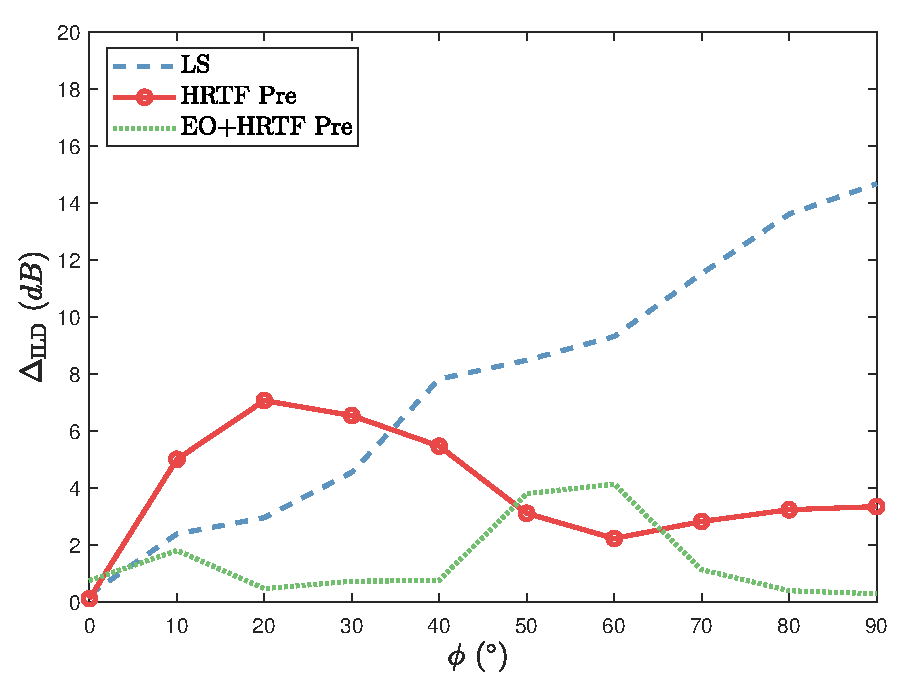
\includegraphics[width=0.48\textwidth]{error_ILD_xiaoshengshi_eigenmike_phiChange_whitenoise}}
\vfill
\subfigure[]{
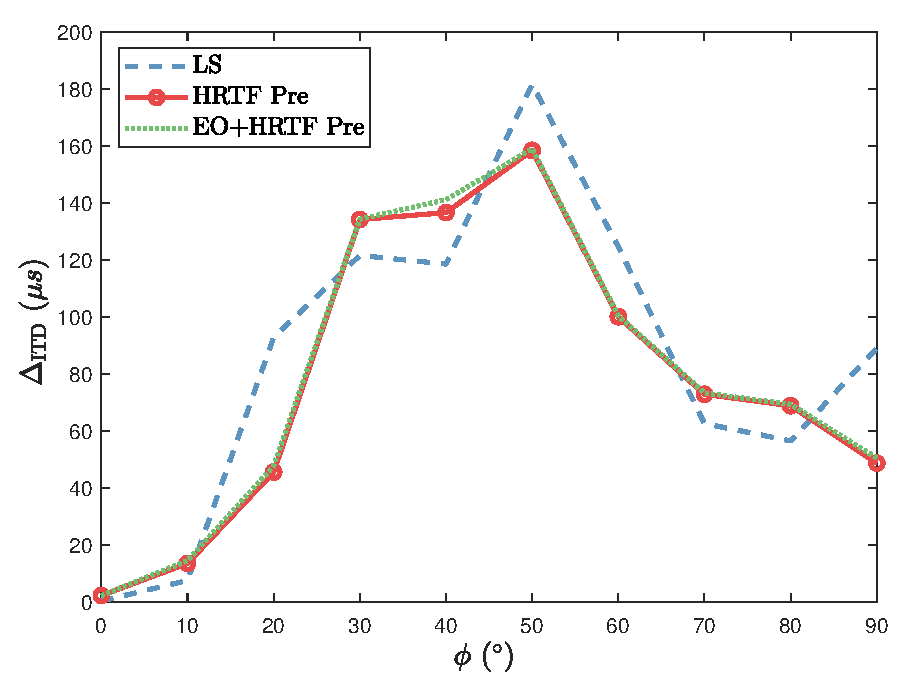
\includegraphics[width=0.48\textwidth]{error_ITD_xiaoshengshi_eigenmike_phiChange_audio}}
\hfill
\subfigure[]{
\includegraphics[width=0.48\textwidth]{error_ILD_xiaoshengshi_eigenmike_phiChange_audio}}
\caption{消声室环境下两种声源信号在不同方位角处的实验结果:白噪声:~(a)~ITD;(b)~ILD;语音:~(c)~ITD;(d)~ILD}
\label{fig.xiaoshengshi_eigenmike_phiChange_whitenoise}
\end{figure}


从图~\ref{fig.xiaoshengshi_eigenmike_phiChange_whitenoise}~可以看出:
\begin{inparaenum}[(1)]

\item 无论是白噪声信号还是语音信号,LS、HRTF Pre~和~EO + HRTF Pre~算法的~$\Delta_{\text{ITD}}$~结果基本一致,这是因为~HRTF Pre~算法进行相位对准的起始频率为~1.5~kHz,EO + HRTF Pre~算法在引入声场扩阶的过程中,当~$N_{T}>N_{s}$~时才开始进行处理,根据~$N_{T} =k R_{T}=2\pi f R_{T}/c$,$R_{T}=0.1$~米和原有声场阶次~$N_{s}=4$~阶可知,进行声场扩阶的起始频率为~2.7~kHz。而评价指标~ITD~的关注频率范围为~1.5~kHz~以下,此频段内~HRTF Pre~和~EO + HRTF Pre~算法并未对双耳信号进行任何处理,因此三种算法的~$\Delta_{\text{ITD}}$~结果没有区别。

\item 无论是白噪声信号还是语音信号,EO + HRTF Pre~算法的~$\Delta_{\text{ILD}}$~结果最小,并且在任意方位角下均可达到较小的误差。LS~算法与~Original~的差距最大,且随着方位角的变化,误差一直增大。

\item 相较于~LS~算法,HRTF Pre~算法在大多数方位角下的~$\Delta_{\text{ILD}}$~有所降低,更加接近~Originial~算法,但是在部分角度($10^{\circ}$、$20^{\circ}$)HRTF Pre~算法的误差大于~LS~算法,进一步分析发现~HRTF Pre~算法在这些角度出现~ILD~的正负错误,可能会带来少量的声源定位错误,而改进方法~EO + HRTF Pre~并未出现此问题。

\item 相比于白噪声信号,语音信号的~ITD~和~ILD~结果有少许变化,这是因为语音信号的能量主要集中在低频,并且在各频点上的能量分布不均,而白噪声在整个频谱上均匀分布,避免了计算波动。但是两种声源类型对应的综合结论一致。

\end{inparaenum}

上图展示了~1.5~kHz~到~8~kHz~频段内平均~ILD~的结果,接下来以方位角~$\phi=40^{\circ}$~为例,对三种算法所获取的双耳信号与参考信号在~8~kHz~以下频段内单个频点处的~$\Delta_{\text{ILD}}$~结果进行展示,如图~\ref{fig:xiaoshengshi_eigenmike_40du}~所示。

\begin{figure}[!h]
\centering
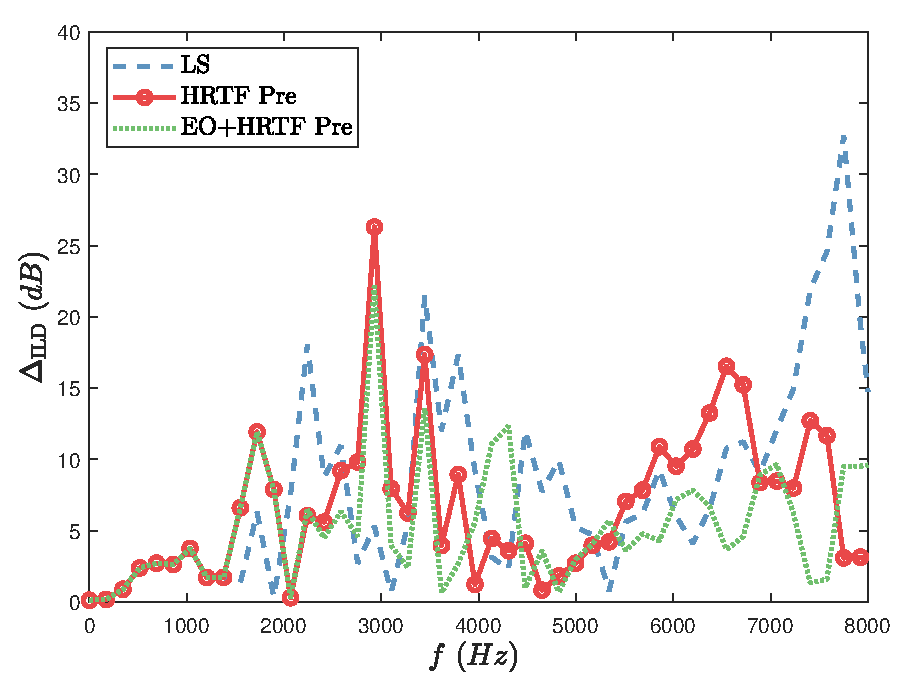
\includegraphics[width=0.6\textwidth]{error_xiaoshengshi_eigenmike_40du}
\caption{消声室情况下方位角~$\phi=40^{\circ}$~时单个频点处的~$\Delta_{\text{ILD}}$~结果}
\label{fig:xiaoshengshi_eigenmike_40du}
\end{figure}

从图~\ref{fig:xiaoshengshi_eigenmike_40du}~可以看出:

\begin{inparaenum}[(1)]

\item 综合整个频段来看, EO + HRTF Pre~算法的~$\Delta_{\text{ILD}}$~结果最小,尤其是在~5~kHz~以上的高频,现有的研究表明,ILD~是高频定位因素,1.5~kHz以上~ILD~才开始对定位起作用,频率大于~4~kHz~时,ILD~才是方向定位的主要因素。HRTF Pre~算法次之,LS~算法的~ $\Delta_{\text{ILD}}$~最大,与图~\ref{fig.xiaoshengshi_eigenmike_phiChange_whitenoise}~中~1.5~kHz~到~8~kHz~频段内平均~$\Delta_{\text{ILD}}$~的结论一致。

\item 相比于~LS~算法,HRTF Pre~和~EO + HRTF Pre~算法的~ILD~开始在~1.5~kHz~有所调整。相比于~HRTF Pre~算法,EO + HRTF Pre~算法的~ILD~开始在~2.7~kHz~有所调整,与图~\ref{fig.xiaoshengshi_eigenmike_phiChange_whitenoise}~的讨论中频率相关的结论一致。
\end{inparaenum}





\subsection{空心球与刚性球的性能对比}\label{subsec.open_rigid}

仿真环境为消声室环境,麦克风阵列采用含有~32~个麦克风的空心球阵,对应的球谐函数分解阶次~$N_{s}=4$~阶。空心球阵的半径从~0.01~米到~0.1~米均匀取值,间隔为~0.01~米。麦克风阵列和声源位于同一水平面,俯仰角为~$\theta=90^{\circ}$,且相距~2~米,声源位于麦克风阵列的正右方,即方位角~$\phi=90^{\circ}$。
声源信号包括两类,白噪声信号和语音信号。

不同声源类型(白噪声、语音)、不同麦克风阵列半径~$R$~对双耳信号的影响如图~\ref{fig.xiaoshengshi_eigenmike_r_eigChange_whitenoise}~所示,其中图~(a)~和图~(b)~是声源为白噪声信号,采用不同麦克风阵列半径时三种算法对应的双耳信号与参考双耳信号之间的~$\Delta_{\text{ITD}}$~和~$\Delta_{\text{ILD}}$~结果,图~(c)~和图~(d)~是声源为语音信号,采用不同麦克风阵列半径时三种算法的~$\Delta_{\text{ITD}}$~和~$\Delta_{\text{ILD}}$~结果。

\begin{figure}[!h]
\centering
\subfigure[]{
\includegraphics[width=0.48\textwidth]{error_ITD_xiaoshengshi_eigenmike_r_eigChange_whitenoise}}
\hfill
\subfigure[]{
\includegraphics[width=0.48\textwidth]{error_ILD_xiaoshengshi_eigenmike_r_eigChange_whitenoise}}
\vfill
\subfigure[]{
\includegraphics[width=0.48\textwidth]{error_ITD_xiaoshengshi_eigenmike_r_eigChange_audio}}
\subfigure[]{
\includegraphics[width=0.48\textwidth]{error_ILD_xiaoshengshi_eigenmike_r_eigChange_audio}}
\caption{空心球情况下两种声源信号在不同麦克风阵列半径时的实验结果:白噪声:~(a)~ITD;(b)~ILD;语音:~(c)~ITD;(d)~ILD}
\label{fig.xiaoshengshi_eigenmike_r_eigChange_whitenoise}
\end{figure}

从图~\ref{fig.xiaoshengshi_eigenmike_r_eigChange_whitenoise} ~可以看出:
\begin{inparaenum}[(1)]

\item 无论是白噪声信号还是语音信号,LS、HRTF Pre~和~ EO + HRTF Pre~算法的~$\Delta_{\text{ITD}}$~结果完全一致,与图~\ref{fig.xiaoshengshi_eigenmike_phiChange_whitenoise}~的讨论一致。并且当麦克风阵列半径接近人头尺寸时,$\Delta_{\text{ITD}}$~达到较小的值。

\item 无论是白噪声信号还是语音信号,HRTF Pre~和~ EO + HRTF Pre~算法的~$\Delta_{\text{ILD}}$~结果远小于~LS~算法,且~ EO + HRTF Pre~算法更适合半径较小的空心球阵(小于等于~0.05~m),HRTF Pre~算法更适合尺寸较大的麦克风阵列。

\item 当麦克风阵列半径~$R$~大于等于~0.05~m~时,声场扩阶算法开始不起作用,甚至对~ILD~有一定的损伤,$\Delta_{\text{ILD}}$~大于~HRTF Pre~算法。这是因为空心球阵情况下会存在球贝塞尔函数零点问题,零点的引入会对声场扩阶算法中的球谐域~MUSIC~定位算法有影响,导致错误的声场扩阶。

\item 半径~$R=0.1$~米时,HRTF Pre~和~EO + HRTF Pre~算法的~$\Delta_{\text{ITD}}$~和~$\Delta_{\text{ILD}}$~结果完全一致,这是因为~EO + HRTF Pre~算法的目标球体半径~$R_{T}=0.1$,此时两种算法等效。

\end{inparaenum}

对球贝塞尔函数的零点进行进一步分析,图~\ref{fig.xiaoshengshi_r_eig_bessel_zero}~给出了~EO + HRTF Pre~算法在不同麦克风阵列半径下三种算法所获取的双耳信号与参考信号在~8~kHz~以下频段内单个频点处的~ILD~结果,以及~4~阶球贝塞尔函数~$j_{4}(kR)$~在不同半径~$R$~下随频率~$f$~的变化情况。

\begin{figure}[H]
\centering
\subfigure[]{
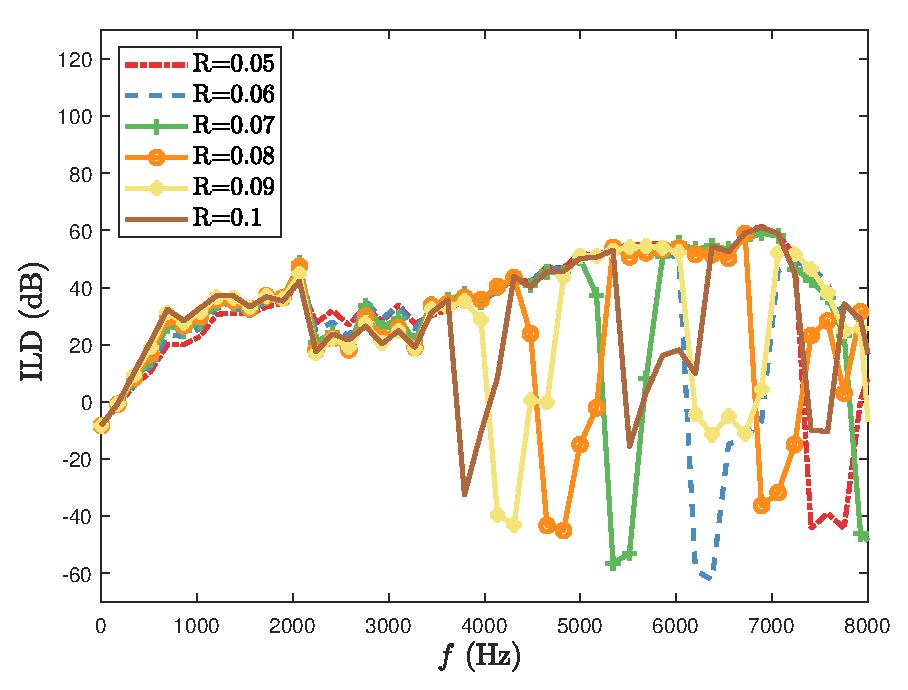
\includegraphics[width=0.48\textwidth]{xiaoshengshi_r_eig_bessel_zero}}
\hfill
\subfigure[]{
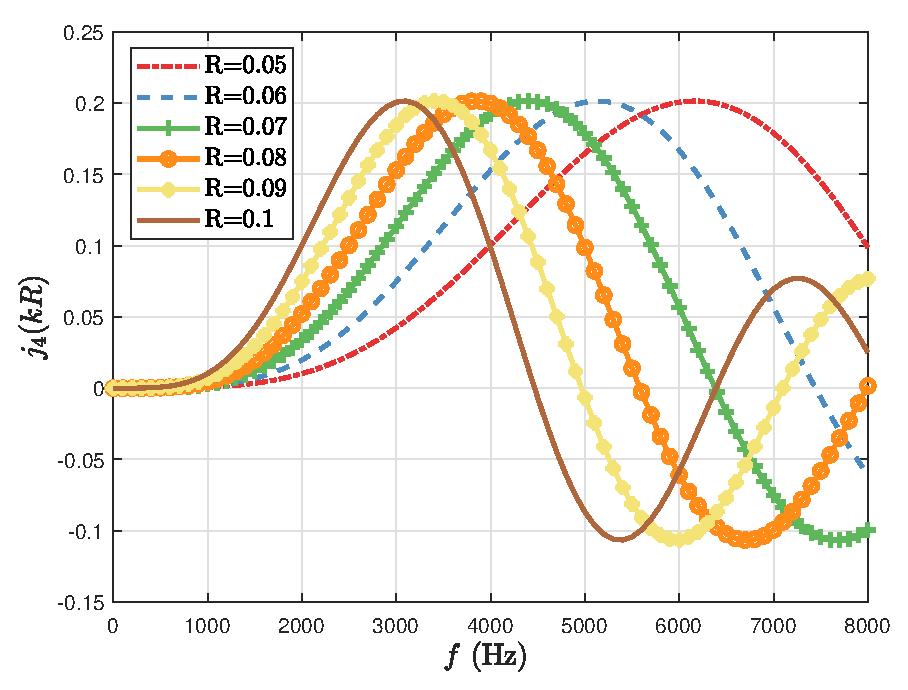
\includegraphics[width=0.48\textwidth]{bessel_4order}}
\caption{消声室情况下不同麦克风阵列半径在各个频点的~ILD~}
\label{fig.xiaoshengshi_r_eig_bessel_zero}
\end{figure}

从图~\ref{fig.xiaoshengshi_r_eig_bessel_zero}~可以看出:

\begin{inparaenum}[(1)]

\item 本实验中声源的方位角~$\phi=90^{\circ}$,ILD~应该为正值,而图~(a)~中部分频率的~ILD~出现负值,且其绝对值较大,严重影响了平均~ILD~结果,因此导致了图~\ref{fig.xiaoshengshi_eigenmike_r_eigChange_whitenoise} (b)~和~(d)~中的~ILD~损伤现象。

\item 对比图~(a)~和图~(b)~可以看出,固定麦克风半径~$R$,ILD~出现错误的频率位于该半径下球贝塞尔函数的零点处或零点附近,这是因为零点的存在导致球谐域~MUSIC~定位算法的错误,从而导致~ILD~错误。

\item 图~(b)~中,对于~4~阶球贝塞尔函数来说,$R\geq0.05$~时,零点开始出现在~8~kHz~以下的频段,且半径~$R$~越大,开始出现零点的频率越小,8~kHz~以下的频段零点出现的次数越多。这也导致了半径越大, EO + HRTF Pre~算法的~ILD~结果与~Original~算法的差距越大。
\end{inparaenum}



在第~\ref{section_microphone_array_coe}~节中对空心球和刚性球进行了详细讨论,并且已经从原理上证明,由于散射声场的存在,刚性球可以避免球贝塞尔函数的零点问题,从而解决空心球带来的一些问题,更加适用于实际系统。

接下来采用刚性球阵进行仿真实验,其余实验设置均保持不变,并且只关注~ EO + HRTF Pre~算法出现~ILD~损伤的情况,即麦克风阵列半径从~0.05~米到~0.1~米均匀取值,间隔为~0.01~米。
图~\ref{fig.rigid_xiaoshengshi_r_eig_whitenoise}~给出了刚性球情况下,不同声源类型和不同麦克风阵列半径下三种算法对应的双耳信号与参考双耳信号之间的~$\Delta_{\text{ITD}}$~和~$\Delta_{\text{ILD}}$~结果,图~\ref{fig:xiaoshengshi_rigid_ILD_fre}~给出了~EO + HRTF Pre~算法在采用不同麦克风阵列半径的刚性球情况下,三种算法所获取的双耳信号与参考信号在~8~kHz~以下频段内单个频点处的~ILD~结果。

\begin{figure}[H]
\centering
\subfigure[]{
\includegraphics[width=0.48\textwidth]{error_ITD_rigid_xiaoshengshi_r_eig_whitenoise}}
\hfill
\subfigure[]{
\includegraphics[width=0.48\textwidth]{error_ILD_rigid_xiaoshengshi_r_eig_whitenoise}}
\vfill
\subfigure[]{
\includegraphics[width=0.48\textwidth]{error_ITD_rigid_xiaoshengshi_r_eig_audio}}
\hfill
\subfigure[]{
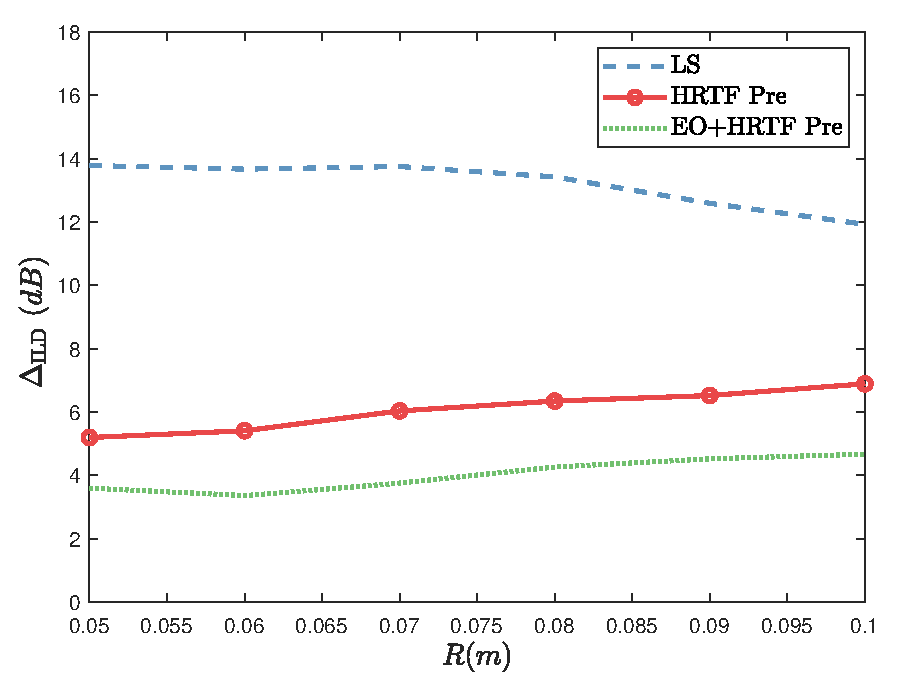
\includegraphics[width=0.48\textwidth]{error_ILD_rigid_xiaoshengshi_r_eig_audio}}
\caption{刚性球情况下两种声源信号在不同麦克风阵列半径时的实验结果:白噪声:~(a)~ITD;(b)~ILD;语音:~(c)~ITD;(d)~ILD}
\label{fig.rigid_xiaoshengshi_r_eig_whitenoise}
\end{figure}

\begin{figure}[H]
\centering
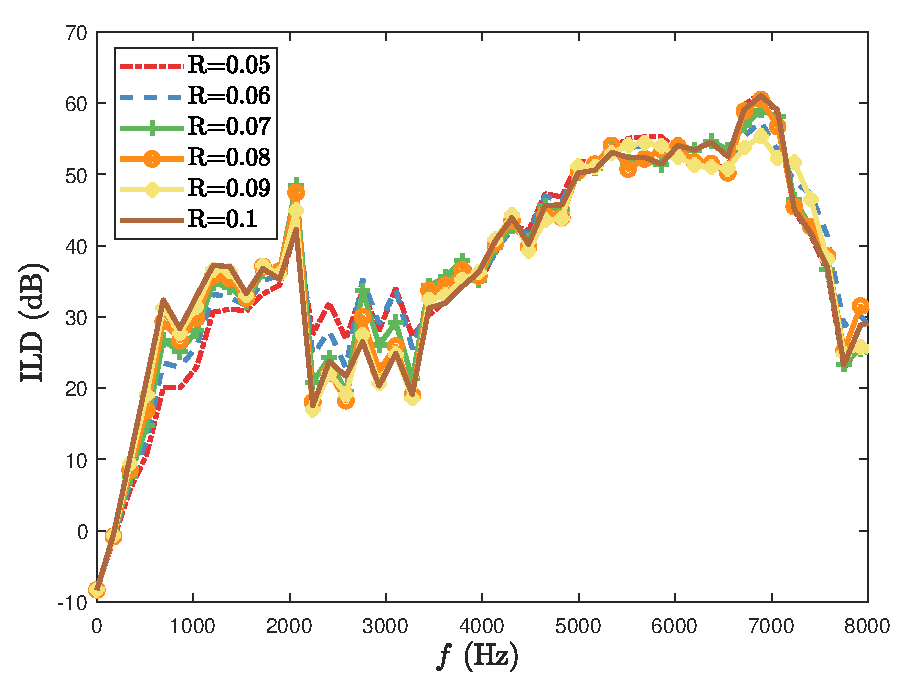
\includegraphics[width=0.6\textwidth]{xiaoshengshi_rigid_ILD_fre}
\caption{刚性球情况下采用不同麦克风阵列半径的单频点~ILD~结果}
\label{fig:xiaoshengshi_rigid_ILD_fre}
\end{figure}


从图~\ref{fig.rigid_xiaoshengshi_r_eig_whitenoise}~和~\ref{fig:xiaoshengshi_rigid_ILD_fre}~可以看出:

\begin{inparaenum}[(1)]

\item 无论是白噪声信号还是语音信号,刚性球情况下~EO + HRTF Pre~算法在各个半径的~$\Delta_{\text{ILD}}$~结果最小,HRTF Pre~算法次之,LS~算法的误差最大,且远大于~HRTF Pre~和~EO + HRTF Pre~算法。

\item 刚性球的使用避免了~EO + HRTF Pre~算法在空心球情况中较大的麦克风阵列半径下的~ILD~损伤现象,因此~EO + HRTF Pre~算法在刚性球情况下适用于研究范围内的任意半径。

\item 对比图~\ref{fig.xiaoshengshi_r_eig_bessel_zero}(a)~和~图~\ref{fig:xiaoshengshi_rigid_ILD_fre}~可以看出,刚性球可以避免球贝塞尔函数的零点给~EO + HRTF Pre~算法带来的~ILD~正负错误,体现了刚性球的优越性。

\end{inparaenum}

\subsection{混响环境下各算法性能对比}

本实验的仿真环境为混响环境,声源在混响室的传播可以用镜像模型方法(Image Source Method,ISM)产生~\tcite{1979Image}。
镜像模型方法通常以矩形结构房间为基本模型,可通过调节墙壁反射系数~$\beta$、房间尺寸大小、声源位置及麦克风接收位置等参数来获得房间冲激响应,目前已经广泛应用于各种仿真实验中。其基本思想是用虚拟镜像来等效地替代声源在墙壁发生的反射,进而确定反射声的传播路径,一旦确定房间设置(尺寸、反射系数)及声源与麦克风的位置,既可计算所有的镜像声源坐标和对应的能量衰减系数。

反射系数的取值范围是~$0$~到~$1$~之间,本文选取的反射系数为~$0$、$0.3$、$0.5$~和~$0.7$,分别对应无混响、低混响、中等混响和强混响的声学环境。混响的强弱也可以用混响时间~$T_{60}$~这一指标来描述,其表示的是在扩散声场中当声源停止后从初始的声压级衰减~60~dB~时所对应的时间,描述了室内混响声的衰减快慢。
常用的两个计算公式为艾润公式和赛宾公式~\tcite{book_xiebosun}:
\begin{align}
T_{60} & = 0.161 \frac{V}{-S ~\text{ln}(1-\alpha)} \nonumber\\
T_{60} & = 0.161 \frac{V}{S \alpha}
\end{align}
其中,$V$~为房间的体积,$S$~为总的吸声面积,$\alpha$~为平均吸声系数,$\alpha = 1-\beta^{2}$,$\beta$~为反射系数。

混响环境下~IACC~是一个重要评价指标,因此本实验中同时使用双耳时间差~ITD、双耳声级差~ILD~和双耳互相关系数~IACC~这三个评价指标对各种算法进行分析。和~$\Delta_{\text{ITD}}$、$\Delta_{\text{ILD}}$~类似,引入~$\Delta_{\text{IACC}}$:
\begin{align}\label{eq.delta_IACC}
\Delta_{\text{IACC}} &= \left|~\text{IACC}_{\text{case}} - \text{IACC}_{\text{Original}} ~\right|
\end{align}
其中,case~表示~LS、HRTF Pre~和~EO+HRTF Pre。

本实验选取尺寸为~$5~\mathrm m\times7~\mathrm m\times3~\mathrm m$~的房间,反射系数为~$0$、$0.3$、$0.5$~和~$0.7$。麦克风阵列采用~Eigenmike~球阵,其包含~32~个麦克风,对应的球谐函数分解阶次~$N_{s}=4$~阶,半径为~0.042~米。Eigenmike~位于房间中心,与声源处于~$z=1.5$~米的同一水平面上,且相距~2~米。声源位于麦克风阵列的正右方,即方位角~$\phi=90^{\circ}$。
声源信号包括两类,白噪声信号和语音信号。

不同声源类型(白噪声、语音)、不同反射系数对双耳信号的影响如表~\ref{tab:ITD}、\ref{tab:ILD}~和~\ref{tab:IACC}~所示,分别为三种算法对应的双耳信号与参考双耳信号之间的~$\Delta_{\text{ITD}}$、$\Delta_{\text{ILD}}$~和~$\Delta_{\text{IACC}}$~结果。表~\ref{tab:IACC}~中的~JND~为参考双耳信号~Original~的~IACC~对应的最小可觉差,参见式~\eqref{eq.JND_IACC}。

\begin{table}[H]
  \centering
  \caption{两种声源信号在不同反射系数下的~$\Delta_{\text{ITD}}~(\mu s)$~}
  {\zihao{5}
    \begin{tabular}{m{3cm}<{\centering}m{1cm}<{\centering}m{1cm}<{\centering}m{1cm}<{\centering}m{1cm}<{\centering}m{0.2cm}<{\centering}m{1cm}<{\centering}m{1cm}<{\centering}m{1cm}<{\centering}m{1cm}<{\centering}}
    \toprule[1.5pt]
     & \multicolumn{4}{c}{白噪声信号}~ & & \multicolumn{4}{c}{语音信号} \\
    \cmidrule{2-5}  \cmidrule{7-10}
    反射系数                    & 0 & 0.3  & 0.5 & 0.7 & & 0   & 0.3  & 0.5 & 0.7 \\ \hline
    LS            & 67 & 26  & 12  & 7   & & 163 & 12   & 6   & 4 \\ \hline
    HRTF Pre      & 66 & 27  & 14  & 8   & & 123 & 34   & 12  & 5 \\ \hline
    EO+HRTF Pre   & 66 & 27  & 14  & 7   & & 124 & 33   & 12  & 5 \\
    \toprule[1.5pt]
    \end{tabular}%
  }
  \label{tab:ITD}%
\end{table}%

从表~\ref{tab:ITD}~可以看出:无论是白噪声信号还是语音信号,三种算法在各个反射系数下的~$\Delta_{\text{ITD}}$~基本一致,语音信号情况下三种算法之间的误差相对较大,这是因为语音信号在各频点上的能量分布不均导致的计算波动。整体结论与之前的实验一致,HRTF Pre~和~EO+HRTF Pre~算法并未对~LS~算法的~ITD~加以改变。


\begin{table}[H]
  \centering
  \caption{两种声源信号在不同反射系数下的~$\Delta_{\text{ILD}}~(dB)$~}
  {\zihao{5}
    \begin{tabular}{m{3cm}<{\centering}m{1cm}<{\centering}m{1cm}<{\centering}m{1cm}<{\centering}m{1cm}<{\centering}m{0.2cm}<{\centering}m{1cm}<{\centering}m{1cm}<{\centering}m{1cm}<{\centering}m{1cm}<{\centering}}
    \toprule[1.5pt]
     & \multicolumn{4}{c}{白噪声信号}~ & & \multicolumn{4}{c}{语音信号} \\
    \cmidrule{2-5}  \cmidrule{7-10}
    反射系数                    & 0     & 0.3   & 0.5   & 0.7  & & 0     & 0.3   & 0.5   & 0.7 \\ \hline
    LS            & 14.8  & 9.3   & 6.4   & 3.6  & & 14.3  & 6.1   & 3.2   & 3.4  \\ \hline
    HRTF Pre      & 3.4   & 3.9   & 3.6   & 1.9  & & 5.8   & 2.1   & 1.9   & 0.7 \\ \hline
    EO+HRTF Pre   & 0.5   & 0.6   & 0.7   & 0.8  & & 4.6   & 0.4   & 2.1   & 1.9 \\
    \toprule[1.5pt]
    \end{tabular}%
  }
  \label{tab:ILD}%
\end{table}%


\begin{table}[H]
  \centering
  \caption{两种声源信号在不同反射系数下的~$\Delta_{\text{IACC}}$~}
  {\zihao{5}
    \begin{tabular}{m{3cm}<{\centering}m{1cm}<{\centering}m{1cm}<{\centering}m{1cm}<{\centering}m{1cm}<{\centering}m{0.2cm}<{\centering}m{1cm}<{\centering}m{1cm}<{\centering}m{1cm}<{\centering}m{1cm}<{\centering}}
    \toprule[1.5pt]
     & \multicolumn{4}{c}{白噪声信号}~ & & \multicolumn{4}{c}{语音信号} \\
    \cmidrule{2-5}  \cmidrule{7-10}
    反射系数                    & 0       & 0.3     & 0.5     & 0.7     & & 0       & 0.3     & 0.5     & 0.7 \\ \hline
    LS            & 0.2866  & 0.0775  & 0.0172  & 0.0017  & & 0.1066  & 0.0176  & 0.0040  & 0.0005  \\ \hline
    HRTF Pre      & 0.1897  & 0.0319  & 0.0076  & 0.0095  & & 0.0589  & 0.0018  & 0.0008  & 0.0011 \\ \hline
    EO+HRTF Pre   & 0.1866  & 0.0467  & 0.0028  & 0.0071  & & 0.0947  & 0.0153  & 0.0031  & 0.0001 \\ \hline
    JND           & 0.2847  & 0.0955  & 0.0260  & 0.0070  & & 0.1049  & 0.0220  & 0.0085  & 0.0070 \\
    \toprule[1.5pt]
    \end{tabular}%
  }
  \label{tab:IACC}%
\end{table}%

从表~\ref{tab:ILD}~可以看出:
\begin{inparaenum}[(1)]

\item 无论是白噪声信号还是语音信号,相较于~LS~算法,HRTF Pre~算法和~EO+HRTF Pre~算法的~$\Delta_{\text{ILD}}$~明显降低。

\item 对于白噪声信号,EO+HRTF Pre~算法的~$\Delta_{\text{ILD}}$~最小,小于~1~dB,HRTF Pre~次之,LS~算法的误差最大。 对于语音信号,不同混响情况下,HRTF Pre~和~EO+HRTF Pre~算法的差异不大。ILD~是一个高频定位因素,因此相对来说白噪声下的结果更为可靠,即~EO+HRTF Pre~算法最优。

\end{inparaenum}


从表~\ref{tab:IACC}~可以看出:
\begin{inparaenum}[(1)]

\item 无论是白噪声信号还是语音信号,在大多数混响环境下(反射系数为~0.7~除外),相较于~LS~算法,HRTF Pre~和~EO + HRTF Pre~算法的~$\Delta_{\text{IACC}}$~有所下降。

\item 反射系数为~0.7~时,对于白噪声信号,HRTF Pre~和~EO + HRTF Pre~算法的~$\Delta_{\text{IACC}}$~与~JND~基本一致,且大于~LS~算法。对于语音信号,三种算法的~$\Delta_{\text{IACC}}$~均远小于~JND。
    但是无论是白噪声信号还是语音信号,其~$\Delta_ {\text{IACC}}$~的数值都很小,$10^{-3}$~量级,可以认为三种算法在空间感上的差异性很小。

\end{inparaenum}

综上所述,HRTF Pre~和~EO+HRTF Pre~算法均对~LS~算法加以提升,EO+HRTF Pre~算法对~HRTF Pre~算法在大多数情况下加以提升,部分情况下保持不变。并且本文所提出的算法~EO+HRTF Pre~在任意混响条件下均可达到好的效果。



\section{本章小结}

本章主要对所提出的双耳渲染算法进行评估。首先介绍了双耳信号的三个评价指标及其计算方法,包括用于评估声源定位精度的双耳时间差~ITD~和双耳声级差~ILD,以及用于评估空间感知的双耳听觉互相关系数~IACC。

实验方面,从消声室和混响室两种环境对算法进行评估。消声室情况下首先探索了不同声源方位和声源类型对双耳信号的影响,结果表明,两种声源信号下,本文所提出的双耳渲染算法在声源位于任意方位角的情况下均可达到较小的误差。
接下来对使用不同阵列半径的空心球和刚性球进行双耳渲染的性能加以对比,详细阐述空心球存在的零点问题及其对定位算法带来的影响,证明了刚性球的优越性。结果表明,空心球只适用于半径较小的球体,以避免球贝塞尔零点出现在关注频段内,而刚性球在任意半径下均可达到最小的误差。
最后在不同的混响环境和不同声源类型下,对三种双耳渲染算法进行对比分析,结果表明,本文所提出的双耳渲染算法在多种混响情况下均能达到较好的效果。